\documentclass[11pt,a4paper]{article}
\usepackage[latin1]{inputenc}
\inputencoding{latin1}
\usepackage[T1]{fontenc}
\usepackage{amsmath}
\usepackage{amsfonts}
\usepackage{amssymb}
\usepackage{graphicx}
\usepackage{verbatim}
\usepackage{multicol}
\usepackage{setspace}
\usepackage{makeidx}
\usepackage{epigraph}
\usepackage{hyperref}
\onehalfspacing
\usepackage[french]{babel}
\usepackage{fullpage}
 %\voffset=-2.5cm
 %\hoffset=-2cm
% \textwidth=17cmrr
 %\textheight=24.5cm
 \newcommand{\til}{TaxIPP-Life}

\author{B�atrice Boutchenik et Alexis Eidelman\\ IPP}
\title{Micro-simulation sur le cycle de vie :\\ le mod�le TaxIPP-Life}


\begin{document}
\maketitle

\begin{center}
Document extr�mement pr�liminaire. Ne pas diffuser, ne pas citer.  \newline \newline
Ce document pr�sente le mod�le \til. La construction de ce mod�le a d�but� il y a moins d'un an au moment de la r�daction de ce rapport. Le mod�le est encore dans une phase de d�veloppement. Les r�sultats du mod�le correspondent pour l'instant plus � des exercices de test qu'� des statistiques. 
\end{center}


\newpage
\tableofcontents
\newpage

\section*{Introduction}
L'objet du projet TaxIPP-Life, débuté en septembre 2012, est la réalisation d'études sur la population française portant sur l'ensemble du cycle de vie. Le regard que l'on porte sur les inégalités peut se voir modifié dans cette optique. Sur des données administratives suédoises, \cite{Bjorklund2011} montre que l'état de pauvreté sur le cycle de vie est temporaire alors que les personnes en haut de la distribution des revenus y restent. Les aller-retours de part et d'autres du seuil de pauvreté est aussi un phénomène connu en France. 
Se pose alors la question de la redistribution sur le cycle de vie. Cette question est en général étudiée sur une base annuelle. Si cette démarche est intéressante pour considérer l'état de la population à un instant donné, elle est souffre de plusieurs limitations. 
D'abord l'estimation de la pauvreté et de la richesse est établie à partir de la situation d'une année seulement et uniquement en fonction des revenus. Ainsi seront pratiquement toujours pauvres les étudiants et souvent le seront les retraités. Si l'on pense que la consommation peut être lissée au cours de la vie et que le revenu permettant d'apréhender cette consommation est le revenu permanent. Une étude annuel ne peut être satisfaisante. Par exemple, un retraité aura en général moins de revenu que lorsqu'il est actif, cependant son niveau de vie a probablement été surestimé lorsqu'il était actif car il a épargné en pensant à sa retraite et est sous-estimé car il peut consommer plus que ses revenus une fois inactif. 
La question du patrimoine est elle aussi primordiale dans l'étude des inégalités. Il est en effet raisonnable de croire qu'un individu ayant un capital (éventuellement un capital attendu à travers un héritage) n'aura pas la même attitude de consommation qu'une personne qui n'en a pas. Si on pense à deux étudiants, l'un aidé par ses parents, l'autre non, dans l'imaginaire collectif celui aidé par ses parents est plus aisé que l'autre. Pourtant, si pour subvenir à ses besoin le second travaille en même temps que ses études, il sera paradoxalement considéré comme plus riche.
 
Le premier point pour justifier une approche sur cycle de vie est donc que l'on peut mieux appréhender la situation des individus. Un deuxième est que si l'on veut étudier la progressivité des transferts ou du système socio-fiscal dans son ensemble, une étude en coupe souffre de limitation importante. 
En effet, les études en coupe doivent contourner la difficulté causée par les transferts dits assuranciels (assurance chômage, retraite et maladie). Ces assurances ne peuvent être vues uniquement comme des transferts. Celui qui cotise ouvre un droit pour plus tard, c'est le principe de l'assurance. Par sa cotisation, il s'assure un revenu futur ou du moins l'espérance d'un revenu. Une étude de la redistribution sur cycle de vie permet d'intégrer ces transferts assuranciels dans l'étude alors qu'ils doivent exclus d'une étude en coupe. Pour ces transferts, comme pour les autres, on est capable d'identifier une redistribution individuel temporelle et une redistribution entre agent. On sépare ainsi la partie d'un prélèvement qu'un individu va \og récupérer \fg \ ou qui lui a été avancée de la partie qui bénéficiera vraiment à d'autres. Pour les prestations, on peut aussi isoler ce qui relève purement de la solidarité de la partie de la prestation que l'individu a lui-même financée \\

L'étandue des questions auxquelles TaxIPP-Life est très grande. On ne les détaillera pas ici car l'état actuel du projet ne permet pas encore d'aborder ces points. Le présent document détaillera essentiellement la méthode utilisée et donnera de premiers résultats provisoires.\\

L'étude sur le cycle de vie exige, et c'est une lapalissade, des données sur l'ensemble de ce cycle de vie. Cela n'est pas sans poser de problème. Le plus évident est que lorsque l'on interroge un individu, il ne connait pas son avenir. Le modèle \til \ contient un module réalisant une projection à un niveau individuel du futur. Ceci sera développé dans la deuxième partie de ce document. La première s'attardera sur un point moins évident qui est que le passé des individus n'est pas non plus si bien connus. En dehors des effets de mémoire qui font qu'une partie du passé est oubliée, aucune enquête ne demande à un individu l'ensemble de ses revenus passés. Des données administratives semblent être la seule solution pour connaitre par exemple la trajectoire professionnelle des individus. Mais les données administratives ne sont pas non plus une panacée, elles ne donnent en général pas d'information sur la vie matrimoniale des personnes, or, savoir qui vit avec qui est déterminant pour étudier la consommation et les niveaux de vie. Enfin, une troisième voie serait l'utilisation d'un panel qui suivrait les individus tout au long de leur vie, toutefois une telle base de données, avec des informations assez riches pour pouvoir appliquer la législation socio-fiscal n'existe pas. Nous avons donc procédé à un matching statistique de données d'enquête et de données administratives. La première partie de document présentera ce matching avec entre les données de l'enquête patrimoine et les données de l'échantillon EIR-EIC.


\section{Construction de la base de donn�es}

\section{Construction de la base de donn�es}

\subsection{Appariement statistique des donn�es EIC-DADS avec l'Enqu�te Patrimoine}

Un des int�r�ts majeurs de TAXIPP Life r�side dans l'utilisation de trajectoires salariales effectivement observ�es, plut�t que simul�es. Les donn�es administratives des EIC et DADS ont �t� utilis�es � cette fin. Celles-ci ont �t� coupl�es � l'enqu�te Patrimoine afin de disposer d'un certain nombre d'informations, notamment au niveau du m�nage plut�t que de l'individu. Un appariement statistique a donc �t� effectu� entre les deux sources de donn�es : appariement statistique exact sur un certain nombre de variables consid�r�es au moment de l'enqu�te (sexe, �ge, PCS � 1 chiffre, tranche de revenus salariaux et de remplacement), puis appariement avec le plus proche voisin, en particulier en termes de trajectoire vis-�-vis de l'emploi.\\

Il a �t� dans un premier temps n�cessaire de manipuler les fichiers EIC-DADS (et UNEDIC) d'une part et l'enqu�te Patrimoine d'autre part afin de les rendre plus exactement comparables quant aux variables utilis�es pour l'appariement statistique : il faut en effet que ces variables soient d�finies de la fa�on la plus proche possible dans une base et dans l'autre. En particulier, il a fallu utiliser l'information des fichiers EIC-DADS-UNEDIC afin de retracer les trajectoires vis-�-vis de l'emploi, selon les m�mes modalit�s que celles renseign�es dans le calendrier r�trospectif de l'Enqu�te Patrimoine, calendrier renseignant les changements entre des situations ayant dur� au moins un an.

\subsubsection{Mise en forme des fichiers EIC-DADS-UNEDIC}

On conserve uniquement les individus n�s � partir de 1942, les donn�es concernant les g�n�rations 1934 et 1938 n'�tant pas compl�tes.

\paragraph{Reconstitution des trajectoires vis-�-vis de l'emploi}
Les observations du fichier DADS correspondent au croisement individu x ann�e x entreprise. A partir de ce fichier et pour les ann�es 1976 � 2001, on d�termine le statut de l'individu au 1er janvier de chaque ann�e, en termes d'emploi � temps plein ou temps partiel. Les donn�es du fichier EIC caisse x individu x ann�e permettent par ailleurs de croiser cette information avec le fait que le salari� �tait dans le public, le priv� ou encore �tait ind�pendant pour l'ann�e donn�e. Ces sources permettent de retracer les modalit�s suivantes de la variable de statut vis-�-vis de l'emploi de l'Enqu�te Patrimoine : salari� du public � temps complet, salari� du public � temps partiel, salari� du priv� � temps complet, salari� du priv� � temps partiel et � son compte .
Lorsqu'il y a cumul de plusieurs emplois au premier janvier de l'ann�e, que ceux-ci soient � temps plein ou temps partiel, on consid�re que l'individu travaille � temps plein. Enfin, l'appartenance au public  ou � la cat�gorie des ind�pendants �tant obtenue dans l'EIC gr�ce � l'appartenance � diff�rentes caisses - appartenance dont seule l'ann�e est connue et non les dates exactes au cours de cette ann�e -, on a 2116 individus qui pour au moins une ann�e sont affili�s � la fois � une caisse du public et � une caisse d'ind�pendants. On attribue al�atoirement un des deux statuts � ces individus pour l'ann�e donn�e.

Le fichier UNEDIC permet quant � lui de retracer pour les ann�es 1984 � 2001 et gr�ce au type d'allocation per�ue le fait qu'au 1er janvier de chaque ann�e l'individu soit en situation de ch�mage indemnis� ou non (ch�mage indemnis� seulement jusqu'en 1992), de formation et de pr�retraite. S'il y a cumul de plusieurs allocations dont une de pr�retraite ou de formation au 1er janvier de l'ann�e consid�r�e, on classe l'individu comme �tant plut�t en pr�retraite ou formation. Lorsqu'on a � la fois un statut provenant du fichier DADS et un statut provenant du fichier UNEDIC pour le m�me individu et la m�me ann�e, on conserve le statut DADS.
L'information provenant du fichier EIC caisse x individu x ann�e , compl�t�e par les dates de sortie des fichiers EIC-DADS-UNEDIC, nous permet de retracer les d�parts � la retraite.
Enfin, le calendrier r�trospectif de l'enqu�te Patrimoine comprend une modalit� "succession de courtes p�riodes  (inf�rieures � un an) d'emploi et de ch�mage", qu'il serait dommage d'assimiler al�atoirement � de l'emploi ou du ch�mage, celle-ci nous renseignant sur un type de situation particuli�re vis-�-vis de l'emploi. De telles p�riodes ont ainsi �t� rep�r�es dans le fichier DADS.

\paragraph{Revenus salariaux et de remplacement pour l'ann�e 2001}
On additionne les salaires nets renseign�s dans les DADS et les salaires nets des fonctionnaires de l'Etat donn�s dans la base EIC caisse x individu x ann�e. On prend enfin en compte les revenus de remplacement, que l'on divise par 0,7 afin de comparer des salaires de r�f�rence et non des revenus effectifs, qui nous int�resseraient moins ici : il serait par exemple peu souhaitable d'apparier un individu gagnant 2000 euros mensuels avec un autre gagnant g�n�ralement 3000 euros environ, mais qui l'ann�e consid�r�e se trouve �tre en situation de ch�mage et donc le revenu de remplacement est donc plus proche de 2000 euros.\\





\subsubsection{Mise en forme de l'Enqu�te Patrimoine}

	L'appariement se fera naturellement lorsque l'on disposera du fichier EIC-DADS 2010, mais on matche pour l'instant l'Enqu�te Patrimoine 2009-2010 et l'EIC 2001 en alignant la premi�re sur l'EIC, et en consid�rant donc la situation d'un individu pour l'ann�e 2010 dans l'Enqu�te Patrimoine comme correspondant � celle pour l'ann�e 2001 de l'EIC. Ainsi, on utilise pour l'appariement selon les trajectoires des dates retard�es de 9 ann�es pour l'Enqu�te Patrimoine, ce qui revient � comparer des situations vis-�-vis de l'emploi pour un �ge donn�.
On d�flate par ailleurs les revenus salariaux et de remplacement de l'Enqu�te Patrimoine 2010 par la croissance nominale observ�e des salaires afin qu'ils soient comparables � ceux provenant des fichiers EIC-DADS-UNEDIC en 2001. De m�me que pour les donn�es issues du fichier EIC, on multiplie les revenus de remplacement par un facteur de 0.7 avant de les additionner aux revenus salariaux.

Les donn�es EIC �tant disponibles pour une g�n�ration sur quatre, on regroupe �galement les individus de l'Enqu�te Patrimoine en cat�gories correspondant � quatre ann�es de naissance : les individus de l'Enqu�te Patrimoine n�s entre 1941 et 1944 seront par exemple appari�s avec la g�n�ration n�e en 1942 du fichier EIC, ceux n�s entre 1945 et 1948 avec la g�n�ration 1946, et ainsi de suite. L'�chantillon est donc compos� d'individus n�s entre 1941 et 1972.\\

On conserve pour l'appariement statistique uniquement les individus qui au moment de l'enqu�te ne sont pas agriculteurs ou ind�pendants, et qui dans leur trajectoire r�trospective de l'Enqu�te Patrimoine ont d�clar� au moins une p�riode comme salari� (� temps plein ou temps partiel, dans le public ou le priv�), comme au ch�mage ou en alternance de courtes p�riodes d'emploi et de ch�mage, entre 1984 et 2001. Pour ceux qui n'ont pas connu de tels �pisodes sur cette p�riode, on matche s�par�ment ceux qui en ont connu au moins une sur la p�riode 1976 � 1983. Les autres ne sont donc pas appari�s et se verront attribuer des revenus salariaux nuls entre 1976 et 2001, ce qui est coh�rent leur d�claration dans l'enqu�te Patrimoine.
On dissocie en effet 1976-1983 et 1984-2001 car la variable de statut vis-�-vis de l'emploi ne peut �tre d�finie de la m�me mani�re sur ces deux p�riodes, les donn�es UNEDIC n'�tant pas renseign�es avant 1984.

Enfin, on n'apparie pas pour l'instant les individus � la retraite \footnote{On ne dispose pas de suffisamment d'individus � la retraite dans l'�chantillon EIC 2001 (puisqu'on ne prend en compte que les g�n�rations n�es � partir de 1942).}.



\subsubsection{Appariement des deux bases}

L'appariement est effectu� de fa�on exacte sur les variables de sexe, d'�ge par tranches de quatre ans, de PCS � un chiffre et de revenus salariaux et de remplacement par tranches au nombre de 12, entre les donn�es de l'ann�e 2001 dans le fichier EIC-DADS et celles de l'ann�e 2010 pour l'Enqu�te Patrimoine (ces derni�res �tant r�-�valu�es pour les revenus salariaux et de remplacement). Au sein d'une cellule d'individus poss�dant les m�mes caract�ristiques, on recherche alors un plus proche voisin quant � la trajectoire en termes de statut entre 1984 et 2001, sauf pour les individus n'ayant pas eu de p�riode salari�e ou de ch�mage entre 1984 et 2001, et aux revenus salariaux et de remplacement.

La distance entre trajectoires est calcul�e en sp�cifiant des co�ts de suppression d'un statut - il est ainsi co�teux de passer d'une trajectoire � la trajectoire identique, avec simplement une p�riode en moins ou en plus - et de substitution d'un statut � un autre. Le co�t de suppression est le m�me quel que soit le statut pendant la p�riode supprim�e, mais les co�ts de substitution varient selon le statut que l'on substitue � un autre statut donn� : on doit ainsi d�finir une matrice de co�ts (cf. infra). On n'autorise pas les statuts manquants au cours ou � la fin d'une trajectoire : une p�riode manquante est cat�goris�e comme "Inactif et autres". On autorise par contre les statuts manquants au d�but des trajectoires, c'est-�-dire avant l'entr�e dans une des bases de donn�es, si celle-ci a lieu apr�s 1976. Une trajectoire consid�r�e est ainsi plus courte si elle comporte des statuts manquants au d�but, mais cela n'est pas vrai si elle comporte des statuts manquants au milieu ou � la fin.


\paragraph{D�finition de la matrice de co�ts pour la distance entre trajectoires}
 La distance entre deux statuts est d�finie comme �tant la diff�rence en valeur absolue entre les revenus (d'activit� et de remplacement) m�dians parmi les sous-groupes se trouvant dans chacun des deux statuts, en 2010. On choisit de consid�rer des distances en termes de salaire puisque c'est finalement l'ad�quation de la trajectoire salariale de l'EIC avec la trajectoire salariale r�elle connue par l'individu de l'Enqu�te Patrimoine qui nous importe. Il est �vident que les distances entre statuts en termes de revenus salariaux et de remplacement ont pu varier entre 1984 et 2010, mais il nous faut d�finir une unique matrice de co�ts de substitution.

\paragraph{Poids relatifs de la distance entre les salaires en 2001 et de la distance entre trajectoires}
Diff�rents essais ont �t� effectu�s pour l'appariement afin de d�terminer l'ordre de grandeur du poids qu'il faut attribuer � la distance entre les trajectoires relativement � celle entre les revenus salariaux et de remplacement en 2001. Lorsque l'on augmente le poids relatif attribu� � la distance entre trajectoires, m�me consid�rablement, le pourcentage de statuts qui ne correspondent pas pour une p�riode donn�e entre ce qui est d�clar� dans l'Enqu�te Patrimoine et ce qui est connu � travers l'EIC ne diminue pas beaucoup. Au contraire, la distance moyenne entre les revenus dans l'Enqu�te Patrimoine et dans l'EIC augmente fortement. On choisit donc d'accorder un poids relativement �lev� � la distance entre les revenus en 2001, puisque cela ne d�t�riore pas grandement la qualit� de l'appariement en termes de trajectoires de statuts, tout en am�liorant assez nettement celle en termes de revenus salariaux et de remplacement en 2001.


\subsection{Trajectoires salariales}

\subsubsection{Imputation des ann�es manquantes}

\paragraph{Imputation des ann�es manquantes pour la Fonction Publique d'Etat}
Les ann�es 1979, 1981 et 1987 sont manquantes en totalit� pour la Fonction Publique d'Etat. Dans le fichier EIC, les salaires de ces ann�es ont �t� imput�es en �tudiant la probabilit� d'�tre entr� dans la fonction publique l'ann�e N plut�t que l'ann�e $N+1$ (si l'individu n'�tait pas d�j� dans la base l'ann�e $N-1$). Cette imputation de la pr�sence dans la fonction publique est conserv�e, mais plut�t que de reprendre simplement le salaire de l'ann�e pr�c�dente, on fait en sorte qu'il y ait une augmentation progressive entre les salaires des ann�es $N-1$, $N$ et $N+1$. Plus pr�cis�ment, on veut qu'en moyenne :\\

$W_{N+1} =  W_{N} \ . \ g_{N+1} \ . \ t$

$W_{N}    =  W_{N-1} \ . \ g_{N} \ . \ t$\\

avec $g$ la croissance nominale des salaires dans le priv� et semi-public (donn�es INSEE) et $t$ un facteur de croissance sp�cifique � la fonction publique et constant entre $N-1$ et $N+1$, et que l'on calcule donc comme $t = \sqrt{\frac{W_{N+1}}{g_{N+1} \ . \ W_{N-1} \ . \ g_{N}}}$.

On choisit ensuite d'appliquer ce facteur (multipli� par la croissance nominale) au salaire de l'ann�e $N-1$ lorsque celui-ci existe, et au salaire de l'ann�e $N+1$ dans le cas contraire, et ce si l'individu est pr�sent dans la fonction publique l'ann�e $N$.
Les salaires des ann�es 1976 et 1977 sont connus dans les DADS mais pas dans les EIC pour la Fonction Publique d'Etat (l'appartenance au fichier de paie des agents de l'Etat est par contre connue). On impute pour l'ann�e 1977 le salaire de 1978 d�flat� par la croissance r�elle des salaires dans le priv� et le semi-public si l'individu appartient � la Fonction Publique cette ann�e-l�, et de m�me pour 1976 en utilisant l'ann�e 1977.


\paragraph{Imputation des ann�es manquantes pour le secteur priv�}
Les ann�es 1981, 1983 et 1990 sont enti�rement manquantes dans les DADS. On estime les revenus salariaux pour chacune de ces ann�es gr�ce � des mod�les tobit.
Pour l'ann�e 1981, on estime tout d'abord un mod�le tobit en r�gressant les salaires nets totaux (issus de l'emploi priv�) pour l'ann�e 1980 sur les salaires (issus du priv�) de 1979 et 1978, l'�ge et l'�ge au carr� en 1980, le sexe, et la pr�sence dans une caisse du secteur priv� en 1980 (connue gr�ce au fichier EIC), ce gr�ce � la proc�dure de Heckman. La s�lection se fait sur les m�mes variables, avec en suppl�ment le statut vis-�-vis de l'emploi en 1978 et 1979. Pour cette estimation, on utilise uniquement les individus pour lesquels il existe au moins un salaire strictement positif pour les ann�es 1978, 1979 et 1982.
Le salaire comme variable explicative est renseign� de fa�on cat�gorielle, par l'appartenance � l'un des neuf premiers d�ciles ou aux cat�gories P90-95, P95-99, P99-99.5, P99.5-99.9, P99.9-99.95, P99.95-99.99, et P99.99-100. Le fait de prendre en compte de fa�on fine l'appartenance au haut de la distribution les ann�es pass�es permet par la suite de simuler des salaires suffisamment �lev�s pour l'ann�e en cours. La variable de statut vis-�-vis de l'emploi est celle qui a �t� construite pour l'appariement, et qui reprend une partie des cat�gories de la variable CYACT de l'enqu�te Patrimoine.
Une fois cette estimation effectu�e, on effectue la pr�diction des salaires nets de l'ann�e 1981 ainsi que de la probabilit� d'avoir un salaire positif, � partir des salaires des ann�es 1980 et 1979, de l'�ge et de l'�ge au carr� en 1981, etc. On n'applique cela qu'aux individus pour lesquels au moins l'un des salaires de 1979, 1980 ou 1982 est strictement positif. On impute un salaire nul aux individus dont les salaires de ces ann�es sont tous nuls.

Pour l'ann�e 1990, on transpose la m�me proc�dure en estimant tout d'abord un mod�le tobit r�gressant les salaires de 1989 sur les donn�es de 1987, 1988 et 1991 (et 1989 pour les variables d'�ge et d'appartenance � une caisse du secteur priv�), puis en effectuant la pr�diction des salaires de 1990 � partir des donn�es concernant les ann�es 1988, 1989 et 1992.
On applique la m�me proc�dure pour l'ann�e 1983. Il n'est pas possible d'utiliser l'ann�e 1981 pour l'estimation et/ou la pr�diction, cette ann�e ayant un statut particulier puisqu'elle a elle-m�me �t� imput�e. On estime ainsi l'effet des salaires etc. des ann�es 1980, 1985 et 1986 sur l'ann�e 1984, puis on obtient la pr�diction des salaires de 1983 en utilisant les donn�es de 1979, 1984 et 1985.


\subsection{R�sultats pr�liminaires : description des trajectoires salariales}

\subsubsection{Volatilit� des revenus sur le cycle de vie}

On consid�re ici les trajectoires salariales sur la p�riode allant de 1976 � 2001, dans le but d'examiner les in�galit�s intra-individuelles de revenu sur une partie du cycle de vie. Pour cela, on s'inspire du travail effectu� par Bj�rklund et Palme (1997) dans le cas de la Su�de. Les auteurs utilisent des mesures d'entropie g�n�ralis�es permettant de d�composer les in�galit�s en deux fractions, in�galit�s interindividuelles de revenu total calcul� sur le cycle de vie d'une part, in�galit�s intra-individuelles au cours du cycle de vie d'autre part. Cette mesure des in�galit�s d�pend d'un param�tre d'aversion � la pauvret� : lorsque celui-ci vaut 0 et 1 respectivement, on retrouve l'indice de Theil-L $I_{0}$ et l'indice de Theil $I_{1}$ respectivement. Le premier correspond � un degr� plus grand d'aversion � la pauvret�, accordant une importance relativement plus grande aux revenus tr�s faibles pour une p�riode donn�e. Les formules correspondant � ces deux indices sont les suivantes :\\

$I_{1}=\frac{1}{n}\sum_{i=1}^{n}\frac{y_{i}}{\overline{y}}\text{log}(\frac{y_{i}}{\overline{y}})$\\

$I_{0}=\frac{1}{n}\sum_{i=1}^{n}\text{log}(\frac{\overline{y}}{y_{i}})$\\


avec $y_{i}$ le revenu de l'individu � la p�riode $i$ et $\overline{y}$ son revenu moyen sur le cycle de vie. $I_{0}$ ne peut �tre calcul� que dans le cas o� les revenus sont non-nuls pour tous les individus � toutes les p�riodes. Cela n'est pas le cas pour nos trajectoires salariales. L'indice de Theil $I_{1}$ au contraire peut �tre calcul� m�me lorsque le revenu des individus est nul � certaines p�riodes, en ne prenant pas en compte ces p�riodes dans la somme (on a $ \lim\limits_{y \to 0} y \ \text{log}(y) =0$). On calcule alors un indice de Theil intra-individuel pour chaque individu, sur la p�riode 1976 � 2001 et pour les g�n�rations 1942 � 1958 (la g�n�ration 1958 a entre 18 et 43 ans et la g�n�ration 1942 entre 34 et 59 ans sur la p�riode consid�r�e). Cet indice individuel renseigne sur la volatilit� des revenus sur le cycle de vie.
Bj�rklund et Palme consid�rent quant � eux les revenus  des individus sur une p�riode de 18 ann�es allant de 1974 � 1991, pour une cat�gorie d'individus " �g�s " (ayant entre 33 et 47 ans en 1974) et une cat�gorie d'individus " jeunes " (ayant entre 18 et 32 ans en 1974). Pour chacun de ces deux groupes, ils examinent la corr�lation entre l'indice de Theil intra-individuel (sur le cycle de vie) et le revenu total sur la p�riode consid�r�e. Celle-ci est significativement n�gative, signifiant que les carri�res salariales sont plus instables dans le bas de la distribution. Lorsqu'ils effectuent la m�me analyse quartile par quartile, les auteurs trouvent une corr�lation significativement n�gative pour le premier quartile, mais non significativement diff�rente de z�ro pour les trois quartiles de revenus (sur le cycle de vie) les plus �lev�s.
Toutes g�n�rations confondues (1942 � 1958), on trouve pour les donn�es EIC-DADS une corr�lation entre indice de Theil intra-individuel et revenus salariaux sur le cycle de vie significativement n�gative (au seuil de 1 \%), d'une valeur de -0.48. Lorsqu'on divise la population en quartiles, les r�sultats sont les suivants :\\

\begin{tabular}{|c|c|c|c|c|}
\hline
           &   P0-25 &  P25-50 &  P50-75 & P75-100 \\
\hline
Indice de Theil moyen &       1.95 &       0.67 &       0.28 &       0.23 \\
\hline
Corr�lation avec le revenu total & -0.74 (***) & -0.47 (***) & -0.18 (***) & 0.18 (***) \\
\hline
\end{tabular}\\

\

Et lorsqu'on examine les individus g�n�ration par g�n�ration, et en d�coupant la distribution � un niveau plus fin (particuli�rement pour le haut de celle-ci), on peut figurer graphiquement les indices de Theil moyens par quantile :
\begin{center}
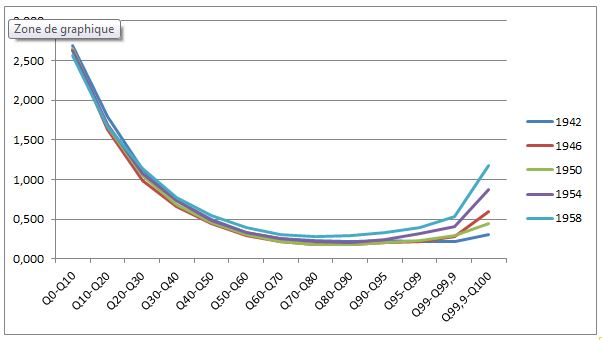
\includegraphics{Theil_intra.jpg}
\end{center}

\
On observe ainsi une baisse de l'instabilit� des revenus salariaux jusqu'� un certain point, et une remont�e assez prononc�e dans l'extr�mit� haute de la distribution des revenus. Ceci pourrait �tre d� en particulier � la prise en compte des bonus et primes dans les salaires, bonus et primes qui sont variables au cours du temps et pouvant repr�senter des montants consid�rables pour les salari�s les plus r�mun�r�s.


\newpage
\section{Simulation sur le cycle de vie}

\epigraph{It's like in chess: First, you strategically position your pieces and when the timing is right you...strike. \\ \textit{David Levinson }\\ \textsc{Independance day}}

Cet �pigraphe est l� pour rappeler que le projet \til~est encore tr�s jeune. Dans une phase de d�veloppement, les r�sultats obtenus ont pour l'instant comme principal voire unique m�rite d'�tre produits par le mod�le. Il s'agit pour l'instant plus d'une r�alisation technique et donc un peu frustrante. La phase de production de r�sultats ne devrait toutefois pas tarder. \\

Avant de commencer cette partie, certaines personnes doivent �tre remerci�es. En effet, le projet \til \ a b�n�fici� de l'aide de plusieurs autres projets. Le souci de partage des personnes concern�es, leur r�ceptivit� aux id�es d'am�lioration ainsi que leurs conseils et leurs temps ont �t� d'une aide extr�mement pr�cieuse. \til~n'est pas encore un sujet abouti mais il serait tr�s �loign� de ce qu'il est maintenant et auraient probablement des objectifs beaucoup plus restreint que ce qu'il a. Je remercie donc l'�quipe d'OpenFisca\footnote{\url{http://www.openfisca.fr/} } et en particulier M. Ben Jelloul, l'�quipe de Liam2\footnote{\url{ http://liam2.plan.be/}} en en particulier G. Dekkers et G. de Menten, l'�quipe Destinie de l'Insee avec Aude Leduc et Anthony Marino et l'�quipe de PensIPP \footnote{\url{http://www.ipp.eu/fr/outils/pensipp-simulation/}} et en particulier D. Blanchet et S.Rabat�.

\subsection{Quelques mots de technique}

Dans cette courte section, seront d�crits les choix techniques faits pour r�aliser la simulation. Nous verrons que la question de la performance ne doit pas �tre n�glig�e. Appliquer la l�gislation socio-fiscale d'une ann�e prend plus de 15 minutes lorsqu'elle est cod�e en SAS par exemple. Dans un calcul sur l'ensemble du cycle de vie, cette l�gislation doit �tre simul�e disons cent fois, l'optimisation du temps de calcul peut donc avoir du bon pour ne pas prendre 25 heures de calcul. Cela d'autant plus que la volont� de travailler sur un gros �chantillon peut augmenter consid�rablement le temps de calcul, et que l'on a l'id�e un jour d'introduire de la d�cision comportementale des agents en fonction de leur esp�rance de gain actualis�e, et donc de simuler la l�gislation encore bien plus de cent fois.

\subsubsection{La base de donn�es initiales}

Comme on peut l'imaginer � la lecture de la premi�re partie de ce document c'est l'enqu�te Patrimoine qui va servir de base d'information � notre mod�le. La raison en est la connaissance des trajectoires professionnelle pass�e. La connaissance du patrimoine est aussi , bien s�r, une des forces de l'enqu�te. On aurait pu utiliser d'autres sources. Par exemple l'enqu�te Sant� et Itin�raire Professionnel, qui comme son nom l� aussi l'indique, est bien moins pr�cise sur le patrimoine mais bien plus sur les conditions de sant�. Pour la simulation du futur uniquement, on peut aussi envisager l'utilisation d'enqu�tes plus g�n�rales et n'ayant pas de volet trajectoire. Ainsi, l'enqu�te Budget des Familles est par exemple attirante car la consommation est alors connue, au moins pour une ann�e. On peut aussi penser � l'enqu�te Logement.
L'id�e est � �tudier mais on peut essayer d'�tendre le matching statistique r�alis� avec deux enqu�tes � plusieurs en constituant ce faisant une sur-enqu�te couvrant la majorit� des champs micro-�conomiques.

Dans la suite, nous ne parlerons que de l'enqu�te Patrimoine 2009-2010. L'�chantillon contient 29 951 individus r�partis en 12788 m�nages\footnote{Les m�nages interrog�s aux Antilles, ont un questionnaire l�g�rement diff�rent. Par souci de simplicit� et pour travailler avec un �chantillon uniforme, ils sont pour l'instant exclus du champ.}. De plus, 14 954 d�clarations fiscales sont imput�es (pour l'instant sommairement).

\subsubsection{La fermeture de l'�chantillon}

Une premi�re limite de l'enqu�te Patrimoine pour notre sujet est qu'elle ne donne pas de lien entre les m�nages. Si les relations sont connues au sein d'un m�nage, on veut aussi conna�tre les relations et particuli�rement les liens de filiation entre les individus qui ne vivent pas dans le m�me m�nage. Cela peut permettre d'imputer ensuite les successions, les pensions alimentaires l'aide pendant les �tudes mais aussi les diff�rentes formes d'aide vers les ascendants, en particulier en cas de d�pendance. On peut aussi imaginer d'imputer un recours aux grands parents pour les gardes d'enfants. \\

Dans l'enqu�te patrimoine, les parents ayant des enfants vivant � l'ext�rieur du domicile se voient poser quelques questions � leur sujet (date de naissance, nombre d'enfant, statut sur le march� de l'emploi, dipl�me, etc.). Nous cr�ons ainsi des individus factices repr�sentant ces enfants hors domicile. Puis par un proc�d� de matching, nous cherchons des individus correspondants, d�clarant un ou deux parents en vie, qui correspondent le plus possible � ces statistiques. On attribue alors les parents enqu�t�s � l'individu fictif comme �tant ses parents

Nous n'utilisons pas les informations ascendantes, celles que les enfants d�clarent � propos de leur parents. Elles sont assez pauvres et concernent pratiquement exclusivement l'enfance de l'enfant or il se peut que la situation des parents ait chang� entre l'enfance de l'enfant et le moment de l'enqu�te. On pourrait aussi utiliser les informations sur le d�c�s ou non des grands-parents. Enfin, notons que nous n'utilisons que les donn�es de l'enqu�te, on n'utilise pas d'information annexe par exemple sur la corr�lation entre les revenus des parents et des enfants. Pour l'instant, on fait donc l'hypoth�se que les variables utilis�es sont suffisantes pour que les distributions crois�es soient respect�es. \\

Nous donnons ici une pr�cision sur la m�thode de calcul pour souligner au lecteur une petite limite actuelle de cette �tape. Lorsque les parents sont interrog�s sur leurs enfants vivant hors du domicile, on leur demande de pr�ciser s'il s'agit de l'enfant du couple ou de l'un d'eux seulement. S'il s'agit de l'enfant du couple, alors on cherche des enfants dont les deux parents sont vivants. Il reste ensuite de tels enfants avec deux parents vivants � apparier ce qui est logique car les parents peuvent �tre vivants et ne plus vivre ensemble. On cherche pour eux, comme pour les enfants n'ayant qu'un parent � trouver, un p�re puis une m�re. Si on ne cherche qu'un parent, il n'y a pas de probl�me. En revanche, un point � noter est que lorsque l'on cherche deux parents, on les cherche ind�pendamment. Par exemple, si on a deux enfants identiques, deux p�res potentiels, l'un de 40 et l'autre de 60 ans et deux m�res potentielles, l'une de 40 ans et l'autre de 60 ans, rien ne contr�le que l'on a plus de chance d'avoir un couple dont les deux membres ont 40 ans et un dont les deux couples ont 60 ans que deux couples avec 20 ans d'�cart d'�ge. On peut donc ne pas reproduire la r�alit� statistique en cr�ant une distribution jointe des parents non r�aliste. Du moins c'est le cas, si on pense que deux couples de parents peuvent avoir des enfants similaires m�me s'ils sont diff�rents au d�part. Une solution serait, une fois la m�re trouv�e, de chercher un p�re avec un �ge assez proche, une autre solution serait de r�aliser un mariage fictif des parents ayant des enfants similaires puis de tirer un couple de parents pour les enfants. \\

Enfin, pr�cisons que le matching est fait � partir d'une m�thode de score (voir Annexe pour plus d'information sur les m�thodes de matching)

\subsubsection{�tendre l'�chantillon}

Travailler avec des pond�rations n'est en g�n�ral pas un probl�me dans le cadre de statistiques statiques. Cependant, dans le contexte particulier de la microsimulation dynamique o� des liens sont �tablis entre m�nages cela pose probl�me. On ne peut en effet pas associer 50 enfants � 3 000 m�res ou unir un homme en repr�sentant 1000 avec une femme repr�sentant 2000 femmes de la population fran�aise. On se demande par exemple, comment on pond�rerait leurs enfants. Pour solutionner le probl�me, le choix a �t� fait de dupliquer les individus autant de fois que n�cessaire pour ainsi avoir une pond�ration uniforme. Dans l'enqu�te Patrimoine 2010, qui contient un sur-�chantillonnage des hauts patrimoines, la plus petite pond�ration est de 6 et cela devrait �tre la pond�ration uniforme. Cela nous m�ne en th�orie � une base de plus de 10 millions de lignes dans la base pour repr�senter la population fran�aise. \\

Le mod�le DESTINIE tire ensuite un sous-�chantillon � partir de cette population �tendue. \til , quant � lui, essaie de tourner sur l'ensemble de cet �chantillon. Cela a aussi l'avantage qu'un m�me individu au d�part se verra associ� � plusieurs carri�res. On conserve ainsi une certaine variabilit� dans le futur de chaque individu de la base initiale ce qui ne peut �tre que bon pour la pr�cision statistique. Comme nous le verrons ci-dessous, travailler sur une base �tendue est un vrai challenge. Pour l'instant, nous travaillons en g�n�ral sur l'�chantillon non �tendu, sans tenir compte des pond�rations dans les diff�rentes �tapes. Une alternative acceptable en termes de temps de calcul et qui permet de tester le mod�le est d'utiliser comme pond�ration uniforme 200, ce qui fait une base de 300 000 individus. Les m�nages avec une pond�ration initiale inf�rieure � 200 se voient attribuer un poids de 200, ce qui biaise donc en th�orie pour l'instant un peu les r�sultats.

\subsubsection{Choix de langage de programmation}

Toutes les �tapes initiales, y compris l'extension de l'�chantillon d�crit ci-dessus, sont r�alis�es en R. Les �tapes de simulation, vieillissement de la population et calcul de la l�gislation sont r�alis�es en Python. On utilise ainsi les forces de chaque programme\footnote{Parce qu'il s'agit d'un matching, l'�tape de cr�ation des liens entre parents et enfants vivant hors domicile est, elle aussi, r�alis�e en Python.}. L'utilisation de Python permet une �criture adapt�e � la microsimulation et est relativement incomparable avec les logiciels statistiques en termes de performances dont on a montr� qu'elles �taient importantes pour \til .
L'�tape de calcul de la l�gislation qui prend 15 minutes en SAS est effectu� dans un temps de l'ordre de grandeur de dix secondes. La possibilit� de travailler avec un gros �chantillon ou avec des �quations comportementales devient envisageable.

\subsection{Les �tapes de la simulation dynamique}

Avant d'entamer cette section, il faut pr�ciser que \til \ est encore un projet jeune en d�veloppement. Les �tapes pr�sent�es ici peuvent toutes �tre am�lior�es, certaines sont tellement rudimentaires qu'elles n'ont d'autre m�rite que d'exister. La description de ces �tapes permet toutefois de donner une premi�re id�e des fonctionnalit�s et possibilit�s de \til . L'�criture sous forme de modules ind�pendants permet � tout moment d'am�liorer chacune de ces �tapes.

\subsubsection{D�mographie}

L'�ge est bien s�r incr�ment� � chaque p�riode.

\paragraph{Naissance} Toutes les femmes en couple �g�es de 16 � 50 ans se voient imputer un enfant\footnote{On �limine les femmes qui ont 8 enfants ou plus ou dont le conjoint est dans cette situation.
On pourrait toutefois supprimer sans difficult� cette condition.}.
Un certain nombre de ces femmes est s�lectionn� en s'assurant de v�rifier les projections de naissance en fonction de l'�ge de la m�re. Le sexe de l'enfant est choisi al�atoirement.

Le fait de ne pas avoir de probabilit� diff�rente pour les femmes selon leurs caract�ristiques autre que leur �ge est probl�matique. Le nombre d'enfants ainsi que le niveau d'�tudes devrait intervenir\footnote{On ne peut pas pour autant dire que le tirage obtenu et compl�tement ind�pendant du niveau d'�tudes et du nombre d'enfants dans la mesure o� ceux-ci interviennent dans les �quations de mise en couple et de divorce, pr�-requis pour se voir imputer des enfants dans \til.}.

\paragraph{D�c�s} La probabilit� de d�c�s ne d�pend que de l'�ge et du sexe. Le nombre de d�c�s pr�dit par les projections d�mographiques de l'Insee est ainsi reproduit. Si une personne d�c�d�e vit seule avec des enfants, ces enfants sont attribu�s � l'autre parent si celui-ci est encore en vie. Si ce n'est pas le cas, ils sont affect�s � un m�nage sp�cial sans adulte avec tous les autres enfants dans ce cas.

\paragraph{Union} Pour l'instant, dans le mod�le, l'union entre deux personnes correspond � la fois � un emm�nagement et � une union l�gale. Sans qu'il n'y ait de contre-indication technique � le faire, il n'y a donc pas de cr�ation de concubinage. Il en existe toutefois dans la base initiale.
Reprenant les �quations utilis�e par DESTINIE � partir du travail de Du�e(??) on impute une probabilit� d'avoir se mettre en couple. Cela est fait d'une part pour les premi�res unions et d'autre part pour les personnes ayant d�j� �t� en couple s�par�ment selon le sexe, en fonction de l'�ge depuis la fin des �tudes, du fait d'avoir un enfant, et de la dur�e depuis la pr�c�dente s�paration le cas �ch�ant. En utilsant une m�thode d'alignement de Liam2 (voir ... ), un tiers de ces personnes est s�lectionn�\footnote{Un calage plus pertinent ne serait pas une mauvaise chose.}. Ensuite, un matching est effectu� pour associer les individus en fonction de leur �ge, de leur diff�rence d'�ge et de leur niveau de dipl�me compar�. Encore une fois, ce matching, crucial pour �tudier bon nombre de questions de redistribution, par exemple, l'impact de l'endogamie, m�riterait d'�tre affin�.
En cas d'union, les personnes rattach�es aux nouveaux conjoints (enfants le plus souvent) emm�nage avec eux. Idem pour les d�clarations fiscales.

\paragraph{S�paration} C'est plus cr�dible cette fois : les s�parations se traduisent � la fois par un changement de logement d'un des deux conjoints et par une rupture du contrat (et donc le passage � des d�clarations fiscales s�par�es). La probabilit� de rupture d�pend du nombre d'enfant du couple, de son anciennet� et de la diff�rence d'�ge entre ses membres. Ceci pourrait �tre r�gi par des probabilit�s mais pour l'instant c'est l'homme qui d�m�nage (sauf lorsque le couple habitait chez ses parents) et la femme qui a une nouvelle d�claration\footnote{Dans le cas de couple homosexuel, le choix est fait al�atoirement}. Les enfants et personnes rattach�es ne changent de logement que s'ils sont li�s � la personne qui part sans �tre li�s � la personne qui reste, que ce soit pour le logement ou pour la d�claration fiscale.

\subsubsection{Logement}
Le travail sur le logement est extr�mement rudimentaire. Les d�m�nagement ne se font que lors des unions et s�parations et lorsqu'une personne de plus de 24 ans n'est ni personne de r�f�rence ni en couple (i.e. vit avec ses parents).
Le travail sur les loyers n'a pas encore �t� fait mais ne devrait pas poser de difficult� majeure.

On pourrait � terme utiliser r�ellement un parc de logement dont on simulerait la variation chaque ann�e. Lors des d�m�nagements, les m�nages choisiraient l'un des logements en fonction de la taille du m�nage et du logement ainsi qu'en fonction des revenus et du loyer. On simulerait ainsi des d�m�nagements en fonction d'un surpeuplement ou sous-peuplement ainsi qu'en cas d'�volution dans les revenus. L'id�e serait de reproduire des tensions sur le march� du logement.

On impute aussi initialement pour chaque logement un propri�taire. Du travail est encore n�cessaire � cette �tape mais indubitablement savoir identifier les propri�taires de leur r�sidence, les locataires sera un plus pour le mod�le.

\subsubsection{March� du travail}

La question de la situation sur le march� de l'emploi est �videmment un �l�ment crucial pour \til , qui veut �tudier la redistribution.
C'est � ce niveau que l'investissement le plus important devra �tre fait. Les �quations de transition devraient �tre estim�es le plus pr�cis�ment possible en tenant compte d'un nombre important de param�tres afin de reproduire la r�alit� du march� du travail.
On est pour l'instant loin d'un niveau satisfaisant mais il sera, l� encore, facile, au moins en termes de programmation d'am�liorer cette partie du mod�le.

\paragraph{�ducation} L'entr�e sur le march� du travail correspond � la fin des �tudes. L'�ge de fin d'�tudes est d�termin� � partir de l'�ge de fin d'�tudes des parents (au moment de la naissance de l'enfant donc). On peut penser � des mod�les plus compliqu�s de d�cision (voir \ref{comportement}). Pour l'instant, on impute pour les individus qui ne sont pas encore sortis du syst�me scolaire un �ge de fin d'�tudes qui est la moyenne de celui de ses parents auxquels on ajoute un �l�ment correcteur en fonction de leur date de naissance pour tenir compte de l'allongement moyen des �tudes.

Lorsque l'individu est encore en �tude, son niveau scolaire est enti�rement d�termin� par son �ge. Ce niveau d'�tude servira ensuite � imputer la valeur du transfert en nature associ�e � l'�ducation.

\paragraph{Statut} Dans l'id�al, on d�termine l'�tat � la date T+1 en fonction de l'�tat � la date T mais aussi des �tats pr�c�dents pour �tre plus pr�cis. Pour l'instant deux m�thodes simplistes ont �t� impl�ment�es. La premi�re calcule un score en fonction de l'�ge puis tire un nombre de transition en suivant des proportions en input du mod�le. La seconde s�lectionne al�atoirement 2,5�\% des individus actifs et inactifs pour les faire changer de statut. Au passage � l'activit�, la cat�gorie d'emploi est tir�e au sort.

\paragraph{Type d'emploi et d'employeur} Comme pour le logement, on cr�e un fichier d'entreprise. Tout est � faire mais on a avec l'enqu�te Patrimoine une id�e de la taille de l'entreprise des salari�s. Une des entreprises peut regrouper les ind�pendants et lib�raux. Cet �l�ment n'est pas prioritaire mais l'id�e est de pouvoir simuler un march� du travail par secteur ou bien d'avoir un mod�le de travailleurs ind�pendants ou encore de se focaliser sur un secteur d'activit� particulier, la m�decine par exemple.

\paragraph{Salaire et revenus} Les salaires sont pour l'instant imput�s � partir d'une �quation de Mincer relativement simple. Si la personne a un revenu d'activit� initialement, on d�termine une productivit� individuelle comme �tant le rapport entre son salaire et le salaire de l'�quation de Mincer. Pour les autres, la productivit� est tir�e al�atoirement. Par la suite, l'�quation de Mincer sera toujours multipli�e par la productivit� pour d�terminer les salaires.

\paragraph{Retraite} Le passage � la retraite est pour l'instant enti�rement d�termin� par l'�ge.


\subsubsection{�pargne et consommation}

Les deux th�mes d'�pargne et de consommation doivent toujours �tre pens�s ensemble. En effet, � chaque p�riode, on sait que le revenu est consomm� ou �pargn�. Si l'un de deux �l�ments est d�termin�, l'autre s'en d�duit. Un taux d'�pargne est donc simul�. Il faut ensuite d�terminer la structure de consommation ainsi que la structure d'�pargne. L'achat immobilier demandera une imputation particuli�re. \\

On se servira de l'enqu�te Budget des Familles, pour imputer une structure de consommation en cat�gorie permettant de calculer les taxes sur la consommation. \\

A partir du nouveau stock d'�pargne de la p�riode T, on d�termine des revenus du patrimoine � la p�riode T+1. Lors du d�c�s d'un individu, on r�partit son capital parmi ses h�ritiers connus dans le mod�le (conjoint, enfants et parents). Si l'individu n'est li� � personne au moment de son d�c�s, on consid�re pour l'instant le capital perdu. Dans un avenir proche, les droits de succession seront aussi calcul�s.

\subsubsection{Calcul de la l�gislation}. En fin de simulation, la l�gislation est calcul�e. Cela inclut les cotisations salariales, l'imp�t sur le revenu, l'imp�t sur la fortune, le bouclier fiscal et les prestations. Les prestations associ�es au handicap sont d�j� simul�es mais cette information n'est pas encore dans la projection de la population. Les taxes (habitation et fonci�re) sont encore � travailler. Tout le volet sant� est aussi � travailler.

Enfin, les retraites et le ch�mage devrait �tre imput�s d'ici peu.

\subsection{Projets futurs}

On a d�j� donn� beaucoup de pistes d'am�lioration dans la section pr�c�dente. Ici, on pr�sente les �l�ments qui pourront agr�menter le mod�le � l'avenir.

\subsubsection{Simulation par mois}

Les mod�les de microsimulation travaillent usuellement sur un base annuelle.
Pourtant la plupart des minima ainsi que les retraites sont calcul�es par trimestre, les prestations familiales et logement ainsi que les cotisations et contributions pr�lev�es � la source sont calcul�es mois par mois. La simulation dynamique �tant rapide, on peut modifier la p�riode pour que le pas devienne le trimestre ou le mois.
L'�tape de mise en couple qui est la plus longue peut �ventuellement n'�tre simul�e qu'une fois par an pour gagner encore du temps de calcul\footnote{Il s'agit l� d'un abus de langage, car si on travaillait par trimestre par exemple, on aura quatre fois un quart des mariages annuels � simuler.
Comme l'algorithme de matching est non lin�aire, il est plus rapide de faire tourner quatre fois sur le quart de l'�chantillon qu'une fois sur l'�chantillon global.
La contrepartie en est que le matching obtenu est th�oriquement de moins bonne qualit� puisque chaque individu n'a qu'un choix limit� d'�poux. Cette partie demanderait � �tre expertis�e.}.
L'application de la l�gislation pourrait se faire d'autant plus pr�cis�ment.

\subsubsection{Transferts interg�n�rationnels}

Dans un premier temps, les calculs sont effectu�s avec une l�gislation fig�e, celle de 2009. Les revenus et la population future sont aussi simul�s en gardant les param�tres de 2009.
Par exemple, il n'y a pas de croissance simul�e. Les revenus pass�s sont eux revaloris� en fonction de la hausse des revenus pour se voir appliquer la l�gislation de 2009. Plus g�n�ralement toutes les �quations pour obtenir des informations non contenues dans la base de d�part sont simul�es � partir des estimations les plus r�centes. Pourtant, les comportements ont chang� (la consommation de t�l�phones portables �tait r�duite dans les ann�es 80 par exemple) et si l'on voulait avoir une repr�sentation fid�le de la consommation pass�e des individus par exemple, il faudrait en tenir compte. \\

Bien �videmment, � terme, \til \ simulera l'ensemble des l�gislations pass�es et simulera la population en fonction de tendances observ�es ou suppos�es. Les imputations d�pendront de la p�riode simul�e. Ceci permettra de reproduire fid�lement la population et de pouvoir proc�der � une analyse d'�quit� interg�n�rationnelle. Pour l'instant, on �tudie finalement une population de 2009 �voluant et ayant �volu� dans les conditions de 2009 hormis pour les trajectoires salariales et matrimoniales avant 2009.

\subsubsection{Comportements}
\label{comportement}

Une dimension suppl�mentaire peut �tre apport�e au mod�le en introduisant des �quations comportementales. Au lieu de simuler des transitions en fonction d'�quations estim�es, on peut cr�er un mod�le d'agent dans lequel les individus prennent leur d�cision en fonction d'anticipation. Il y a deux d�cisions importantes dans le cycle de vie dans lesquelles ces mod�les ont leur place : le choix d'�ducation et la retraite.

Le choix d'�ducation est le plus compliqu� des deux car les anticipations rationnelle portent sur une dur�e plus grande et la diversit� des trajectoires envisag�e peut �tre tr�s importante. L'id�e serait, pour un individu devant d�cider � la p�riode T d'entrer sur le march� du travail ou continuer ses �tudes, de g�n�rer une �valuation de ses revenus dans les deux options et de lui faire choisir celle qui optimise son utilit� (actualis�e).
Ainsi, on pourrait mesurer l'influence d'une hausse de l'imp�t sur le revenu, des minima sociaux ou encore des retraites sur les choix d'�ducation.
Bien s�r, la carri�re n'est pas enti�rement d�termin�e par le choix d'�ducation, on pourra, dans les deux options, simuler plusieurs centaines d'avenirs possibles et estimer ainsi l'esp�rance de l'utilit� de chaque option.

\subsubsection{Autres enqu�tes}

Comme on l'a dit en introduction de cette partie, le mod�le pourrait aussi gagner � utiliser d'autres enqu�tes. En particulier l'utilisation d'enqu�tes portant sur la sant� pourrait ajouter cette dimension au mod�le.


\section{R�sultats pr�liminaires : simulation des allocations familiales (...et de ??)}

\section*{Annexe}

\subsection*{M�thode de matching}

\hspace{-2.5cm}
\begin{tabular}{|p{3.2cm}|p{1.2cm}|p{1.2cm}|p{1.2cm}|p{1.2cm}|p{1.2cm}|p{1.2cm}|p{1.2cm}|p{1.2cm}|p{1.2cm}|p{1.2cm}|}
\hline
           & (1) & (2) & (3) & (4) & (5) &  (6) & (7) & (8) & (9) & (10) \\
\hline
Salari� du public � temps complet (1) &          0 &       8600 &       2900 &      12400 &       5300 &      15120 &      11900 &      19260 &       7100 &      23300 \\
\hline
Salari� du public � temps partiel (2) &       8600 &          0 &       5700 &       3800 &       3300 &       6520 &       3300 &      10660 &       1500 &      14700 \\
\hline
Salari� du priv� � temps complet (3) &       2900 &       5700 &          0 &       9500 &       2400 &      12220 &       9000 &      16360 &       4200 &      20400 \\
\hline
Salari� du priv� � temps partiel (4) &      12400 &       3800 &       9500 &          0 &       7100 &       2720 &        500 &       6860 &       5300 &      10900 \\
\hline
A son compte (5) &       5300 &       3300 &       2400 &       7100 &          0 &       9820 &       6600 &      13960 &       1800 &      18000 \\
\hline
Ch�mage (6) &      15120 &       6520 &      12220 &       2720 &       9820 &          0 &       3220 &       4140 &       8020 &       8180 \\
\hline
Succession de p�riodes d'emploi et de ch�mage (7) &      11900 &       3300 &       9000 &        500 &       6600 &       3220 &          0 &       7360 &       4800 &      11400 \\
\hline
Reprise d'�tudes ou formation (8) &      19260 &      10660 &      16360 &       6860 &      13960 &       4140 &       7360 &          0 &      12160 &       4040 \\
\hline
Pr�retraite (9) &       7100 &       1500 &       4200 &       5300 &       1800 &       8020 &       4800 &      12160 &          0 &      16200 \\
\hline
Inactif et autres (10) &      23300 &      14700 &      20400 &      10900 &      18000 &       8180 &      11400 &       4040 &      16200 &          0 \\
\hline
\end{tabular}

\

Tableau r�sumant la qualit� du matching selon les poids relatifs utilis�s pour les distances ?

\

Tableau d�crivant les salaires imput�s par rapport aux ann�es adjacentes ?

\bibliographystyle{plain}
\bibliography{biblio}



\end{document} 